\documentclass[11pt,a4paper,titlepage]{article}
\usepackage[utf8]{inputenc}
\usepackage[dutch]{babel}
\usepackage{amsmath}
\usepackage{amsfonts}
\usepackage{amssymb}
\usepackage{graphicx}
\usepackage{hyperref}
\usepackage{algorithm}
\usepackage{algpseudocode}\usepackage{float}
\usepackage{fullpage}
\renewcommand{\familydefault}{\sfdefault}

\algblockdefx{ForEach}{EndForEach}[2]{\textbf{for each} #1 \textbf{in} #2 \textbf{do}}{\textbf{end for}}

\author{Pieter-Jan Coenen en Stijn Caerts}
\title{Practicum Toepassingen van Meetkunde in de Informatica \\ Snijdende rechthoeken}
\date{20 mei 2016}

\begin{document}
	\maketitle
	\tableofcontents
	\newpage
	\section{Beschrijving algoritmen}
	\subsection{Algoritme 1}
	\emph{Algoritme 1} is een brute-force algoritme. Elke rechthoek wordt gecontroleerd met elke andere rechthoek voor snijding. Om te vermijden dat we twee rechthoeken dubbel controleren op snijpunten, houden we een lijst bij van de rechthoeken waarvoor we snijpunten met alle andere rechthoeken al zijn nagegaan. In pseudocode ziet dat er uit als volgt.
	\begin{algorithm}[H]
		\caption{}
		\begin{algorithmic}[1]
			\State intersections $\gets \varnothing $
			\State checked $\gets \varnothing $
			\ForEach {rect1} {rectangles}
				\ForEach {rect2} {rectangles}
					\If {rect1 $\neq$ rect2 \textit{and} rect2 $\notin$ checked}
						\State intersections $ \gets $ intersections $ \cup $ calculateIntersections(rect1, rect2)
					\EndIf
				\EndForEach
				\State checked $\gets$ checked $\cup$ rect1
			\EndForEach
		\end{algorithmic}
	\end{algorithm}
	Aangezien we twee geneste lussen hebben, en we niet dubbel controleren voor eenzelfde paar rechthoeken. De functie \emph{calculateIntersections()} wordt daarom $ (n-1) + (n-2) + \dots + 2 + 1 = \frac{n(n-1)}{2} $ keer uitgevoerd en dus heeft \emph{Algoritme 1} een complexiteit van $\mathcal{O}(n^2)$.
	
	\subsection{Algoritme 2}
	\emph{Algoritme 2} is een doorlooplijn-algoritme. Dit betekent dat we de rechthoeken gaan ordenen volgens x-coördinaat en vervolgens deze lijst met rechthoeken doorlopen. De doorlooplijn gaat volgens stijgende x-waarde en als de doorlooplijn een rechthoek snijdt, voegen we die rechthoek toe aan de lijst van actieve rechthoeken. Als de rechthoek niet langer gesneden wordt door de doorlooplijn, verwijderen we de rechthoek weer uit de lijst van actieve rechthoeken. Als we een nieuwe rechthoek tegenkomen, controleren we enkel of er snijding is tussen die rechthoek en de rechthoeken die op dat moment actief zijn. Dit zorgt er voor dat we meestal minder vaak moeten controleren of twee rechthoeken snijden. In de worst case moeten we bij dit algoritme echter ook voor alle andere rechthoeken controleren of er snijding optreedt. Dit is het geval als alle rechthoeken samen actief is.
	\begin{algorithm}[H]
		\caption{}
		\begin{algorithmic}[1]
			\State intersections $\gets \varnothing $
			\State queue $\gets$ priority queue van rechthoeken gesorteerd op de x-coördinaat, initieel van het punt linksonder.
			\State active $\gets \varnothing$
			\While {queue is not empty}
				\State rect1 = queue.poll()
				\If {rect $\notin$ active}
					\State voeg rect toe aan de queue, met de x-coordinaat van het punt rechtsboven als sorteringscriterium.
					\State snijpunten $\gets$ snijpunten $\cup$ alle snijpunten van rect met alle andere rechthoeken die actief zijn
					\State active $\gets$ active $\cup$ rect
				\Else
					\State active $\gets$ active $\backslash$ rect
				\EndIf
			\EndWhile
		\end{algorithmic}
	\end{algorithm}
	
	\subsection{Algoritme 3}
	\emph{Algoritme 3} is gebaseerd op \emph{algoritme 2}, het werkt grotendeels op dezelfde manier. In plaats van op snijding te controleren met alle actieve rechthoeken, controleert \emph{algoritme 3} enkel op snijding met de rechthoek waarvan de onderste zijde het dichtst bij de bovenste zijde van de geselecteerde rechthoek ligt en de rechthoek waarvan de bovenste zijde het dichtst bij de onderste zijde van de geselecteerde rechthoek ligt. Indien er snijding optreedt, herhalen we deze operatie in de desbetreffende richting. Voor snel deze rechthoeken te vinden, maken we gebruik van een Red-Black Tree. In een Red-Black Tree kan je de \texttt{ceiling()} en \texttt{floor()} van een element berekenen in $\mathcal{O}(\log n)$ tijd.
	
		\begin{algorithm}[H]
			\caption{}
			\begin{algorithmic}[1]
				\State intersections $\gets \varnothing $
				\State queue $\gets$ priority queue van rechthoeken gesorteerd op de x-coördinaat van het punt linksonder.
				\State active $\gets \varnothing$
				\While {queue is not empty}
				\State rect1 = queue.poll()
				\If {rect $\notin$ active}
				\State voeg rect toe aan de queue, met de x-coordinaat van het punt rechtsboven als sorteringscriterium.
				\State snijpunten $\gets$ snijpunten $\cup$ alle snijpunten van rect met alle andere rechthoeken die actief zijn
				\State active $\gets$ active $\cup$ rect
				\Else
				\State active $\gets$ active $\backslash$ rect
				\EndIf
				\EndWhile
			\end{algorithmic}
		\end{algorithm}
	
	\section{Experimenten en correctheid}
		\subsection{Experimenten}
		We hebben verschillende experimenten uitgevoerd om de complexiteit en werking van onze algoritme na te gaan. Eerste hebben we een doubeling experiment uitgevoerd waarbij de x- en y-coördinaten van de hoekpunten tussen 0 en 1 liggen.  Nadien hebben opnieuw verschillende doubeling experimenten uitgevoerd waarbij eerst de x- en y-coördinaten van de hoekpunten tussen 0 en 0,2 liggen, daarna tussen 0 en 0.5 en vervolgens laten we de waardes van de hoekpunten variëren tussen 0 en 0.75.
			\subsubsection{Doubeling experiment met hoekpunten tussen 0 en 1}
				We hebben een doubeling experiment uitgevoerd waarbij het aantal rechthoeken laten toenemen vanaf 1 tot 8192.  We hebben hierbij de tijd in miliseconden gemeten die de drie algoritme nodig hebben om de snijpunten van de rechthoeken te vinden.
				\begin{figure}[H]
				\centering
				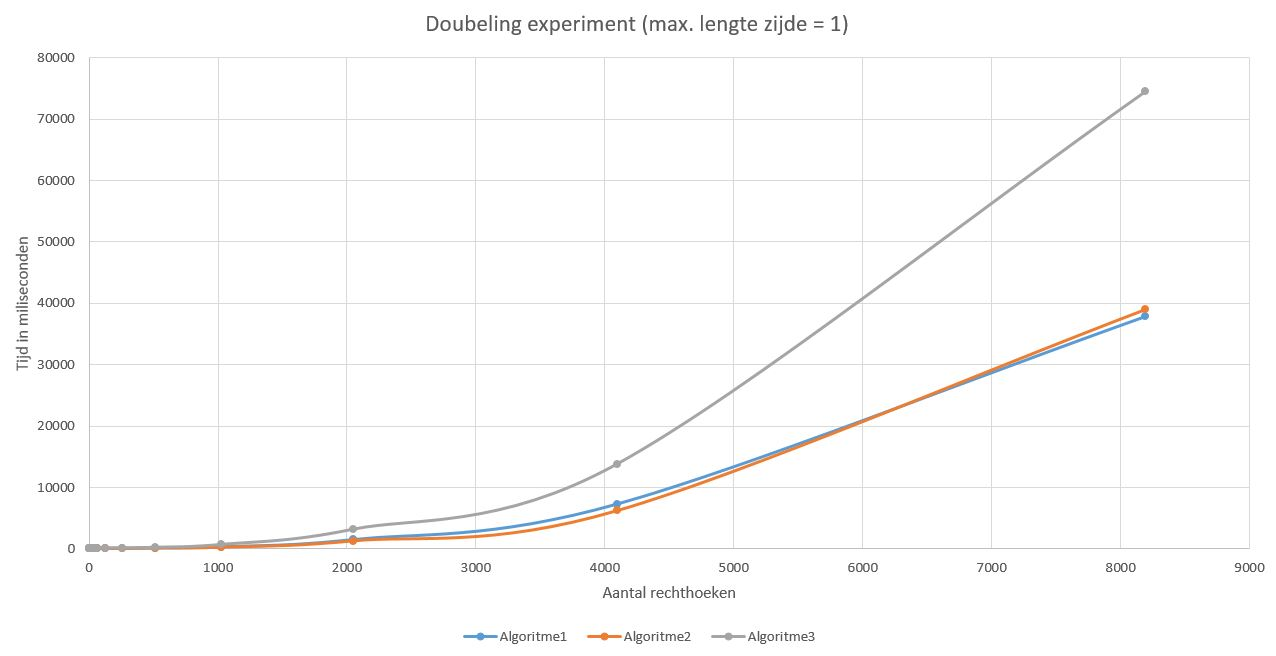
\includegraphics[width=0.75\textwidth]{zijde1.JPG}
				\caption{\label{fig:convR}Grafiek voor het doubeling experiment met zijde die variëren tussen 0 en 1}
				\end{figure}
			\subsubsection{Doubeling experiment voor verschillende lengtes van de zijden}
				Ook hier hebben we een doubeling experiment uitgevoerd.  We hebben hierbij de tijd in miliseconden gemeten die de drie algoritme nodig hebben om de snijpunten van de rechthoeken te vinden. We hebben dit experiment eerst gedaan voor zijdes met een maximale lengte van 0.01, dan voor zijdes met een maximale lengte van 0.1, vervolgens voor zijdes met een maximale lengte van 0.2 en tot slot voor zijdes met een maximale lengte van 0.5.\\ \\
				We verkregen de volgende grafieken:
				\begin{figure}[H]
				\centering
				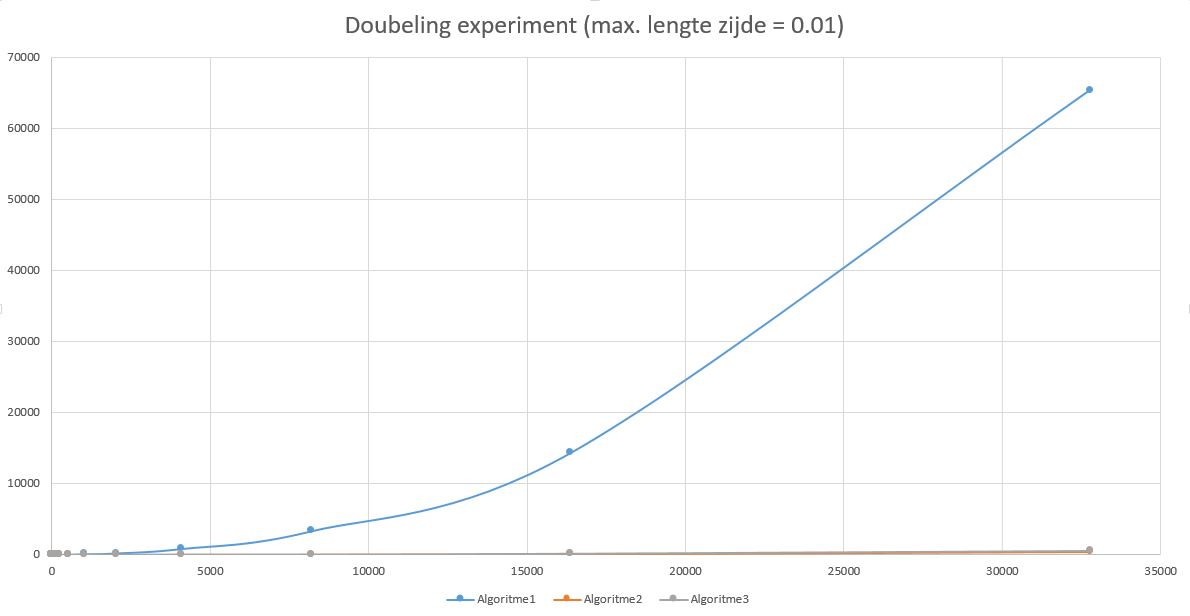
\includegraphics[width=0.75\textwidth]{zijde001.JPG}
				\caption{\label{fig:convR}Grafiek voor het doubeling experiment met zijdes die variëren tussen 0 en 0.01}
				\end{figure}
				\begin{figure}[H]
				\centering
				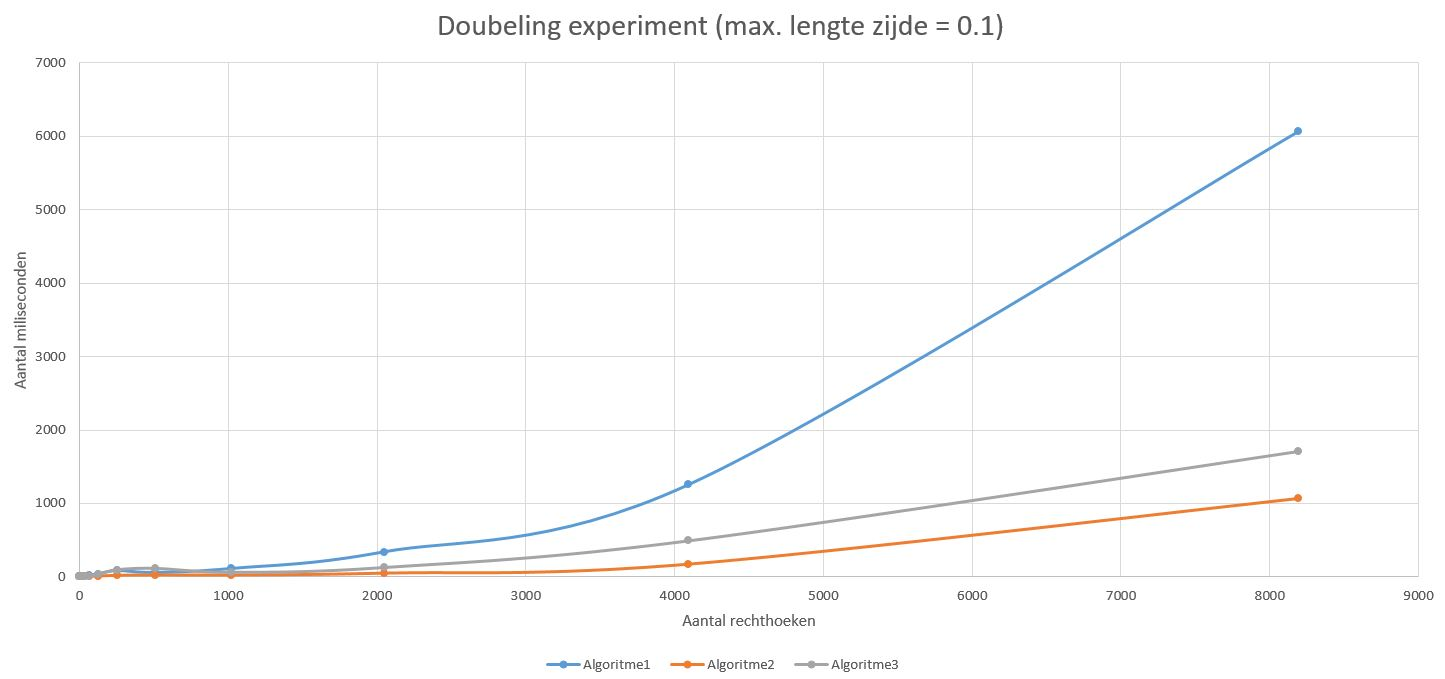
\includegraphics[width=0.75\textwidth]{zijde01.JPG}
				\caption{\label{fig:convR}Grafiek voor het doubeling experiment met zijdes die variëren tussen 0 en 0.1}
				\end{figure}
				\begin{figure}[H]
				\centering
				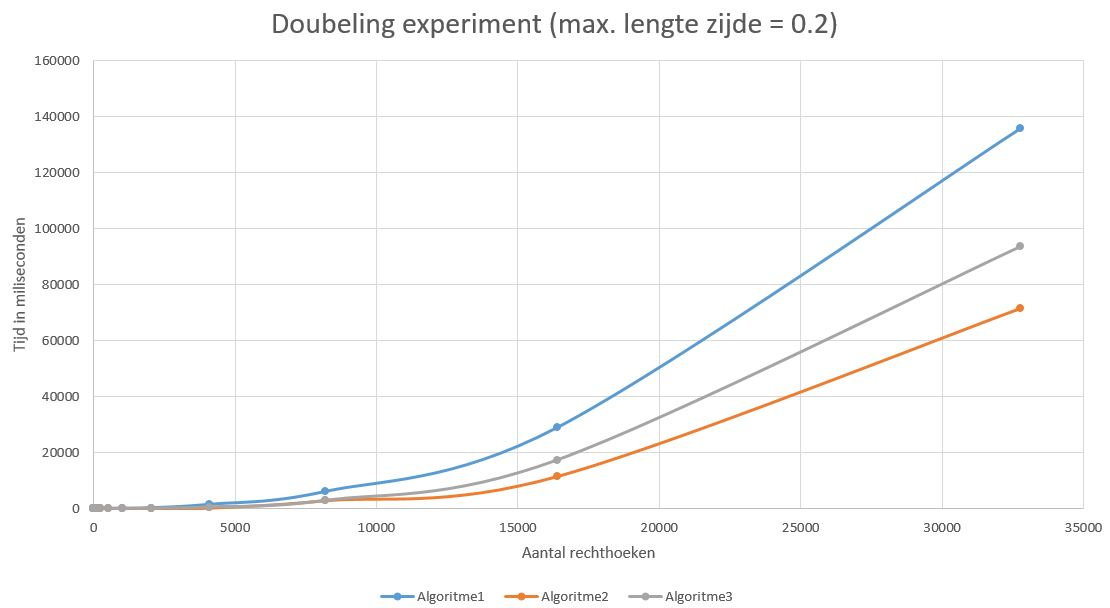
\includegraphics[width=0.75\textwidth]{zijde02.JPG}
				\caption{\label{fig:convR}Grafiek voor het doubeling experiment met zijdes die variëren tussen 0 en 0.2}
				\end{figure}
				\begin{figure}[H]
				\centering
				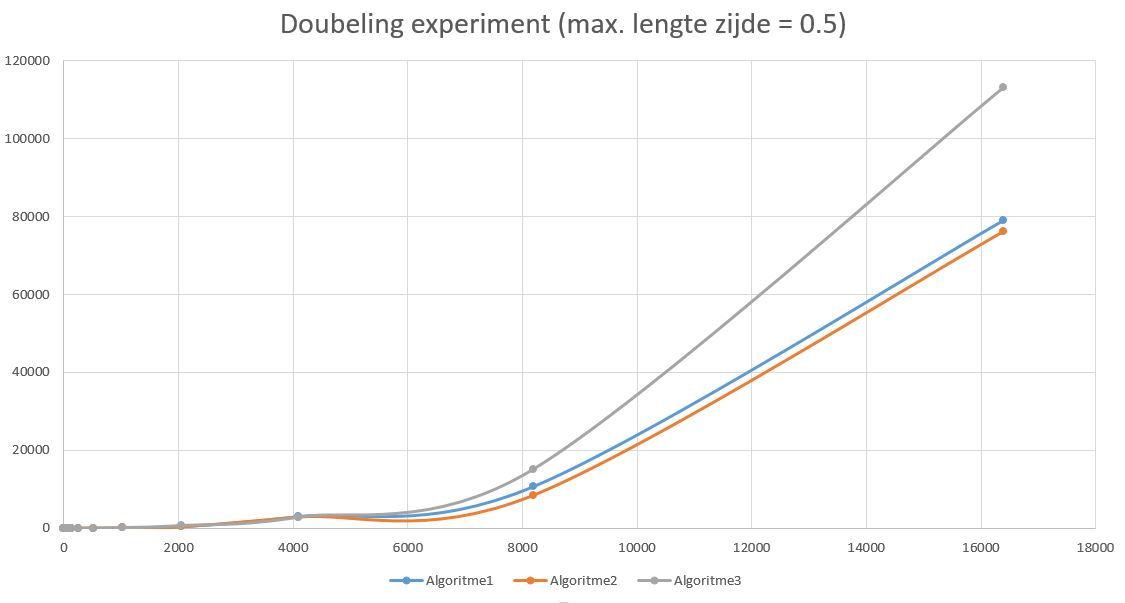
\includegraphics[width=0.75\textwidth]{zijde05.JPG}
				\caption{\label{fig:convR}Grafiek voor het doubeling experiment met zijdes die variëren tussen 0 en 0.5}
				\end{figure}
		\subsection{Correctheid}
			\subsubsection{Algoritme 1}
				Bij algoritme 1 vergelijken we elke rechthoek met elke andere rechthoek, zoals beschreven in vraag 1.  Alle rechthoeken worden dus met elkaar vergeleken voor snijpunten. Om te kijken of twee rechthoeken snijpunten hebben berekenen we eerst de overlappende rechthoek.  Als r1 en r2 twee rechthoeken zijn waarvan we de snijpunten willen vinden, dan bereken we de overlappende rechthoek (r3) met de volgende formule:
					$$r3.Lox = max(r1.Lox, r2.Lox)$$
					$$r3.Loy = max(r1.Loy, r2.Loy)$$
					$$r3.Rbx = min(r1.Rbx, r2.Rby)$$
					$$r3.Rby = min(r1.Rby, r2.Rby)$$
			De punten waar r1 en r2 mogelijk kunnen snijden zijn beperkt tot de vier hoekpunten van r3. Een hoekpunt van r3 kan alleen een snijpunt van r1 en r2 zijn als een van de volgende twee voorwaarden geldt:
				\begin{enumerate}
					\item Als de x-coördinaat van dat r3 hoekpunt een x-coördinaat is van een hoekpunt van r1 en wanneer dat de y-coördinaat van dat r3 hoekpunt een y-coördinaat is van een hoekpunt van r2.
					\item Als de x-coördinaat van dat r3 hoekpunt een x-coördinaat is van een hoekpunt van r2 en wanneer dat de y-coördinaat van dat r3 hoekpunt een y-coördinaat is van een hoekpunt van r1.
				\end{enumerate}
			Alle hoekpunten van r3 die aan deze voorwaarden voldoen zullen snijpunten zijn van de rechthoeken r1 en r2.  \\
			Om deze theorie nog eens te bevestigen hebben we onze resultaten ook nog eens grafisch gecontroleerd. We hebben een 50 tal keer de intersectie punten berekend voor een twintig tal willekeurig genereerde rechthoeken en de resultaten vervolgens grafisch gecontroleerd. Daarnaast hebben we zelf ook enkele randgevallen (zoals rechthoeken waarvan de zijdes samen vallen) bedacht en hiervan de intersectie punten berekend en vervolgens grafisch gecontroleerd. \\
			Aangezien dat onze theorie dus blijkt correct te zijn kunnen we dus veronderstellen dat algoritme 1 correct werkt.
			\subsubsection{Algoritme 2 en 3}
				Aangezien dat we er zeker van zijn dat algoritme 1 correct is hebben we dit ook gebruikt om de correctheid van algoritme 2 en 3 na te gaan.\\
				We hebben de computer in totaal 50 miljoen keer 20 willekeurige rechthoeken laten genereren en de intersectie punten hiervan laten bereken door de drie algoritme. Zowel algoritme 2 als 3 gaven dezelfde resultaten als algoritme 1. \\
				Daarnaast hebben we de computer ook een duizendtal keer 1500 willekeurige rechthoeken laten genereren en vervolgens de intersectie punten berekend met de drie algoritme. Ook voor deze test gaven de drie algoritme dezelfde resultaten.\\
				 Aangezien al deze testen waren geslaagd, kunnen we er vanuit gaan dat algoritme 2 en 3 ook correct werken.
	
				
			
			
	\section{Bespreking resultaten}
	
\end{document}